\documentclass[12pt,letterpaper]{article}

\usepackage{amsmath}
\usepackage{mathrsfs}
\usepackage[pdftex]{color,graphicx}
\usepackage{verbatim}
\usepackage{setspace}
\usepackage{subfig}
\usepackage{algorithm}
\usepackage{algorithmicx}
\usepackage{algpseudocode}

\newcommand{\Eq}[1] {Eq.~(\ref{eq:#1})}
\newcommand{\Fig}[1]{Fig.~\ref{fig:#1}}
\newcommand{\Sec}[1]{Sec.~\ref{sec:#1}}
\newcommand{\Eqs}   {Eqs.~}
\newcommand{\Figs}  {Figs.~}
\newcommand{\Tbl}[1]{Table~\ref{tbl:#1}}
\newcommand{\Etal}  {{\it et al.}}
\newcommand{\Figa}[1]{Fig.~\ref{fig:#1}(a)}
\newcommand{\Figb}[1]{Fig.~\ref{fig:#1}(b)}
\newcommand{\Figc}[1]{Fig.~\ref{fig:#1}(c)}
\newcommand{\Figd}[1]{Fig.~\ref{fig:#1}(d)}

\begin{document}

Here are the comments on the reviews:\\

\textbf{ (2) Is the exposition clear? How could it be improved?} \\

Review \#8: 


The correct definition of Hausdorff distance uses MAX, not SUM as in Equation 3. See
http://en.wikipedia.org/wiki/Hausdorff\_distance . The current $d_H$ is reasonable but is
not Hausdorff.

{\it  - Thanks for pointing this out. The equation 3 is based on the concept of Hausdorff distance 
but not exactly and is suitable for keyslice detection for our approach. 
It would be more appropriate to use another name to avoid any confusion. } \\

line 257: "problem" is unclear.

{\it  - The problem here refers to balance the model accuracy and time-space efficiency.} \\


line 270-271: unclear.

{\it  - Let's say there are 100 vertical slices, like those shown in Figure 7(a). 
Let's assume 10 curvatures are found in each of them, so totally 1000 curvatures are found in all slices. 
Each curvature can be represented by a small range $\delta$. 
Then we will count for each $\delta$, how many curvatures are located at this small range. 
We choose those ranges that contain more than, say 50, as the keyslice location.} \\


Review \#1:


In Equation (1), why are the slabs normalized? It seems to be just for convenience.
This is probably more for ease of implementation, rather than any other reason.

{\it - The purpose of normalization is to keep the ratio in 2D image. Let's say $(X_{max} - X_{min}) = 50.0$,
$(Z_{max} - Z{min}) = 40.0$ and let's assume the image width and height is $W = 1024, H = 392$. Then, we
would mapping the $X$ coordinate to $W$, and $Z$ coordinate to $H$. Without normalization, the ratio will
be changed $(50.0/1024 \neq 40.0/392)$.} \\


Section 4.2, the assumption about only 2D translations can severely constrain the
approach. This will manage to find only symmetry aligned to the axes. In cases, like
castles, etc. such an assumption can be easily violated (for example, rotated towers).
Symmetry based hole filing may still leave significant gaps that can produce artifacts
after BPA. In the present formulation, there is no coupling between adjacent slices.
Using information (as prior) across adjacent slices can help in filling in large holes
(due to occlusion, etc.). 

{\it - The symmetry computation is only an optional step to improve the input data. In some dataset where
the symmetry might only impose little affect on the data improvement, the symmetry computation could
be ignored.
Certainly we can apply more complicated symmetry computation but the overhead is largely increased.
As a lightweight modeling approach, the symmetry computation is largely simplified by only
considering 2D translations. }\\



 Can equation (3) lead to high values in case of missing points (in the slice for $I_r$),
leading to additional slices? 

{\it - Yes, it could. However, it would not affect much if we got more keyslice.}\\


 Figure 11: Is this the top view or the side view? 

{\it - It is a top view of the building. }\\


Lines 459-460, which model are simplified using qslim? For completeness it will be
good to mention how to obtain a model is obtained directly from the point cloud
(Figure 15b). 

{\it - Figure 15a and 15b are simplified using qslim directly from point cloud.}\\


Review \#90:


 Generally clear. No picture taken by normal camera is shown for the scene in Figure
12. People don't know what it is. An odeum? 

{\it - Any picture of Hunter theater? }\\



\textbf{ 4) Could the work be reproduced from the information in the paper? Are all important algorithmic or system details discussed adequately? Are the
limitations and drawbacks of the work clear? }\\

Review \#8:

 The line beautification scheme in lines 320-327 could use additional detail; it was
unclear to me.
Would it be useful to prefer lines that are axis-aligned (with respect to the symmetry
axis)? 

{\it - This beautification scheme can use lines that are axis-aligned as well as other lines detected
by hough transform. Basically this scheme connect all short lines belong to a long line no matter 
what direction these short lines are pointing to.}\\


How exactly is the surface created between adjacent keyslices?
Line 339 explains "the space between each pair of keyslices can be interpolated by the
lower keyslice".
Does this mean that there is no continuous join with the upper keyslice?
Does this result in horizontal gaps in the surface, i.e. lack of watertightness?
For the roof in Figure 10, we see that a horizontal surface is created at the top of
the main building and below the 8 turrets.
When is such a horizontal surface created, and how does it connect with the vertical
surfaces?
Is the resulting surface a manifold?
All these issues are related to the "surfaces from contours" problem. In this work the
"branching" case is handled by introduction of horizontal surfaces, which is
interesting.
This needs a lot more detail. 

{\it - Yes, currently this is no continuous join with the upper keyslice. However,
if we choose a small $\tau_d$ for keyslice detection, the discontinuous join issue
can be hardly observed.}\\


Review \#90:


Line 275: The combination of Hausdorff distance measurement and curvature inference...
How to combine? 

{\it - Basically, it is an union of the results from both Hausdorff distance measurement and 
curvature inference. Let's say the keyslices detected by Hausdorff distance are
 $10, 23, 50, 78, 99$ and the keyslices detected by curvature inference are
$17, 23, 50, 44$. Then, the final keyslices are $10, 17, 2, 50, 44, 78, 99$. }\\


Line 325: We integrate the BPA and HT methods by first applying a dilation operation
on I using 8-connected neighbors to get the dilation image ...
How does the result of BPA fit into this procedure? For the description, we can only
know that HT used the dilation of the image I, which is the original image defined in
Section 4.2. I guess that the author wants to define I as the result of BPA by
removing outlier points? or by linking the points in the circular list. Please clarify
this issue. Dilation by what kernel size? 

{\it - The dilation operation is based on BPA lines as shown In Figure 9(a). The kernel we 
were using is 3x3 (8-connected). }\\


Line 379 As before, the 3D data points inside the range of HR are projected along both
left-right (X axis) and face-inside (Z axis) directions. Then, the keyslice detection
is carried out based on the Hausdorff distance similarity measurement for both
directions.
Which direction first? X or Z? Why? How to get the segmentation as shown in Figure 11? 

{\it- We did X first, then Z. However, the order should not matter. The segmentation
is obtained by similarity measurement as described in Line 375-379.}\\


Experiment: Slices 2D image pixel resolution = ? How sensitive to image pixel
resolution? 

{\it- The resolution is 1024x392. The image pixel resolution will affect the resolution
of the final reconstructed 3D model. But the approach should not be sensitive to 
the image resolution.}\\


\textbf{ 7) Explain your rating by discussing the strengths and weaknesses of the submission. Include suggestions for improvement and publication
alternatives, if appropriate. Be thorough -- your explanation will be of highest importance for any committee discussion of the paper and will be used by
the authors to improve their work. Be fair -- the authors spent a lot of effort to prepare their submission, and your evaluation will be forwarded to them
during the rebuttal period.} \\

Reviewer \#60:\\

It it not clear to me whether the proposed method, which is based on existing work on
2D shape simplification, is the best way to approach the 3D reconstruction problem for
modeling urban buildings. While the decomposition of the point cloud to horizontal
slabs does address the memory issue, solving independent 2D curve reconstruction
problems only takes horizontal smoothness into account. However this fails to take
into account smoothness in the vertical direction. An early commitment is made while
solving the 2D problem which could potentially lead to a bias for models which
resemble a stack of slabs esp. for surfaces which contain curvature in a vertical
plane.

{\it- As mentioned before, if we choose a small $\tau_d$ for keyslice detection, 
vertical discontinuous can be hardly observed. However, for low resolution model,
this is still a limitation and one of our future work. } \\

A comparison with the method of "Variational Shape Approximation" from Steiner et al.
2004 seems like a more appropriate comparison rather than the comparison with Qslim
shown in the paper.

{\it- In fact, our proposed method is capable of surface reconstruction from point clouds
and surface simplification from reconstructed 3D model. Therefore, for comparison, it is
not fair to compare any approach falling only one of the above categories. To do a fair
comparisoin, we first apply 3D BPA algorithm on point clouds to obtain high resolution 3D model, 
and then use this high resolution 3D model as input for QSlim to do the surface simplification
on given number of triangles which are equal to the number of meshes in the models generated by
our proposed method.
Steiner et al. compared their method of ``Variational Shape Approximation'' 
with QSlim, and found that Qslim outperforms their algorithm if a given number of triangles is sought.} \\

The experiments in this paper are limited to one dataset which does not exhibit some
of the complexities that come up in urban modeling. The input point cloud is also
extremely dense and high quality in this case, and the experiments described in the
paper does not convince me whether the method will work as well for noisy, less dense
range scans with larger holes. Some more experiments on a wider set of datasets would
be more convincing.

{\it- we are actively applying the proposed approach on more dataset. 
We will show experimental results on about half dozen of the dataset by the due time of revision version (September 3). 
These dataset include both exterior and interior scans of buildings.}\\


Reviewer \#1:\\

I am curious about how sensitive is the method with respect to finding the major axis
(line 182-183). Slight error can potentially lead to staggered reconstruction (think
of the tower of Pisa).

{\it- The method might be sensitive to the major axis finding. However, the major axises
finding algorithm actually are very reliable and robust. In Appendix, more details are elaborated about
the rectification of the point clouds.} \\

Reviewer \#78:\\

It seems to me that the algorithm looks for one (global) symmetry line,
i.e. one global reflective symmetry, in the model and mirrors all
point along this line. This is not a solution to a general
hole filling problem.
Could you please explain in the rebuttal how that works on
the example in figure 12 that depicts the interior scan?
Where can you put a symmetry plane in this model?
Could you please also explain the following. If windows are the problem
and create missing data point, will not the same areas be missing
in the mirrored second half of the building?

{\it - The symmetry computation is only an optional step to improve the input data. In some dataset where
the symmetry might only impose little affect on the data improvement, like in figure 12, 
the symmetry computation could be ignored.
Certainly we can apply more complicated symmetry computation but the overhead is largely increased.
As a lightweight modeling approach, the symmetry computation is largely simplified by only
considering 2D translations. 
For the window area, the missing data would not matter. What matters is when some part of the builing
is missing due to blocking of the laser beam by some objects in front of it. This missing could be
recovered by symmetry computation.
}\\

I am concerned that the paper and video only contain a single
real example (plus some interior scan, but that is mainly one wall).
How can I know that the parameters of the algorithm work
for a larger class of models? How do I know that the
algorithm itself works for a larger class of models?
What is the class of models that the system works for?
What is a failure example?

{ \it - Again, we are actively applying the proposed approach on more dataset. 
We will show experimental results on about half dozen of the dataset by the due time of revision version (September 3). 
These dataset include both exterior and interior scans of buildings.}\\

Reviewer \#90:\\

1. This paper claim to be an automatic method (such as Line 48 and 83). However, it is
not. Human efforts are needed. For example, human efforts are needed to define inner
and outer boundaries to delete points belong to other objects. Line 191: To tackle
these issues, we define inner and outer bounding boxes for the building to clip away
unrelated scene objects. Line 213: which can be obtained through user input. Line 406:
The chairs and some other fine details were manually culled. If a large manual
interaction time is needed for each building, given the fact that the model quality is
low (discussed below), why do we take the trouble to use this approach instead of
modeling the building by hands in software such as Google Sketchup, where a skill
worker only need one or two minutes?

2. The proposed method relies on many parameters. For example:
a) parameters $\sigma$ in Line 205,
b) threshold $\tau_d$ in Line 247,
c) radius r in Line 296,
d) threshold $\tau_r$ in Line 312,
e) a new set of threshold parameters needed in Line 379-381.
The parameters are no-trivial to determine and vary from one case to another since
they directly affected by the scope of the building. For example, a small house need a
set of parameters. A tall or large building need another set of parameters. A range
scanning for a building at 200 meters distance need a set of parameters, which
scanning at 100 meters distance need another set of parameters. This makes the method
very difficult to be useful in practice.

{\it - First of all, these are simple manual interaction. And second of all, all the manual interactions are optional. 
I dont think Google Sketchup can handle large-scale point cloud dataset and it is non-trivial to get
a high-resolution model from point cloud dataset.
Regarding to the parameters, only $\tau_d$ and $\tau_r$ are important ones, which are used to
get different resolution of the models. Others can be fixed.}\\

4. Low result quality.
The result is far from visual pleasing. In Figure 15, we can see that no matter (c) or
(d) is not good at all, given the fact the range scanning can provide a great detail.
In (c), we can see that the mesh of the wall has many artifacts. It is even worse than
just giving a flat plane. Lots of important details are lost, which makes the
structure of the building become unrealist. For example, the major pattern of windows
in (c) and (d) can not be preserved. An intruded rectangle for a window with simple
mesh is even much better than a complex shape shown in (d).

{\it - For Figure 15(c) and (d), these are low-resolution models. Please refer to 
Figure 1(d) to the final high-resolution model} \\

\section{Appendix}
%%%%%
Although the multiple scans of point cloud data have been registered, 
they are not rectified as depicted in \Fig{pc_orig}. 
Please note the point cloud has been sub-sampling by a factor of 50.
This is not suitable for our further 3D modeling.
As one of the pre-processing steps, this registered data will be rotated
and translated to be aligned with world coordinates.

%% Put the image of rectfied data.
\begin{figure}[htbp]
\begin{center}
\begin{tabular}{c}
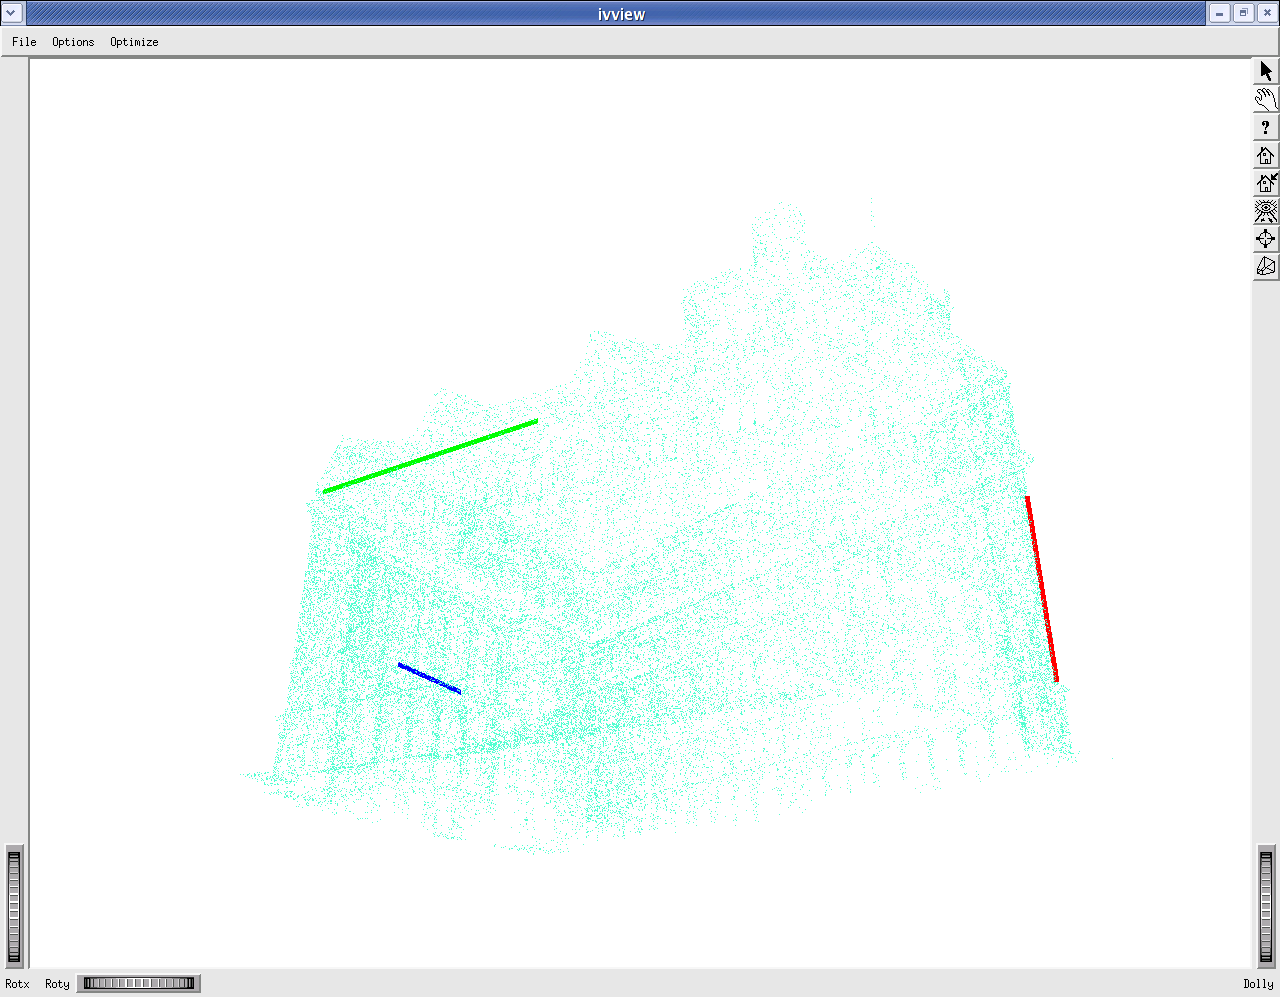
\includegraphics[width=\textwidth]{point_cloud_not_rect.png}
\end{tabular}
\end{center}
\caption{ The registered point cloud without rectification. }
\label{fig:pc_orig}
\end{figure}

As we know, there are a lot of line features existed in the point cloud, which
provides a good clue for rectifing the data. 
For each scan $s$ of the scene, we can obtain a set of line segments $L_s$. 
Assume $T_s$ is the transformation matrix for the scan $s$ to be registered with other scans.
In other words, for any point $P(x,y,z)$ in the scan $s$, $P*T_s$ will transform the
point $P$ into the final registered coordinate system as shown in \Fig{pc_orig}.

We can obtain the major axises by clustering these line segemetns $L_s$ from different
scans. The purpose of clustering is to group the lines whose direction are very close to each other.
To cluster these lines, we first transform the line segments in $L_s$ into world
corrdinate system using $T_s$ as described above. After transformation, we will
get a larger line set $L = {l_1, l_2, \ldots, l_n}$. For each line $l_i$, we first
normalize it to a unit vector:
\begin{equation*}
\bar{l_i} = \frac{l_i}{\parallel l_i \parallel}
\end{equation*}

The unit vector $\bar{l_i}$ has the unique length 1, which provides a good starting point 
for clustering since we do not need to worry the length of the lines. 
An array of bins are used to hold the unit vectors.
As the initial step, the first line $\bar{l}$ is picked up and is insert into the 
first bin and set the counter of the bin to 1.
When a new unit vector $\bar{l_n}$ is observed, we try to see whether there is an
existed unit vector in the bins which has similar direction as $\bar{l_n}$. This is
done by computing the distance $d_{\pm}=\parallel \pm\bar{l_n} - \bar{l_i} \parallel$.
Because $\bar{l_n}$ can has two opposite directions, we can compute both of them and
choose the smaller value as the distance $d$. If $d$ is smaller enough, $\bar{l_n}$
is clusterd with the line $\bar{l_i}$ and the counter of the bin holding $\bar{l_i}$
is increased by 1. On the other hand, if $d$ is big, we have to compare $\bar{l_n}$
with a line in the next bin. If $\bar{l_n}$ could not fit any line in the bins, we
will insert $\bar{l_n}$ into a new bin and set the counter of the bin to 1. 
To avoid the bias of the initial select, each unit vector $\bar{l_i}$ is
adjusted to be the mean of all unit vectors falling inside this bin. 

Once we go through all the lines in $L$, the clustering is complete. 
The next step is to choose the major axises from the clustering results. 
Essentially, this is to choose bins whose counters are among largest. 
Assume $u$, $v$, and $n$ represent the three largest bins. This is demonstrated in
\Fig{pc_orig} in red, green and blue respectively. To rectify the data,
we can refer to the following transformation matrix $\mathbf{M}$:
\begin{figure}[htbp]
\begin{center}
\begin{tabular}{c}
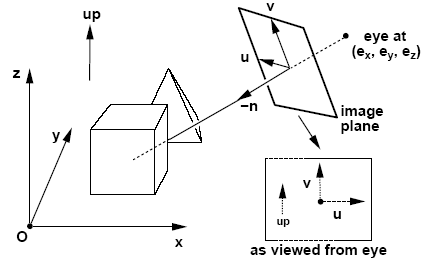
\includegraphics[width=0.5\textwidth]{point_cloud_rect_matrix.png}
\end{tabular}
\end{center}
\caption{ The transformation matrix. }
\label{fig:pc_rect_matrix}
\end{figure}

\begin{equation*}
\mathbf{M} = \left(
\begin{array}{cccc}
u_x & u_y & u_z & -e_x \\
v_x & v_y & v_z & -e_y \\
n_x & n_y & n_z & -e_z \\
  0 &   0 &   0 &    1 
\end{array} \right)
\end{equation*}

This is illustrated in \Fig{pc_rect_matrix}. $(x, y, z)$ is the world coordinate system.
The rectified coordinate system is represented using $(u, v, n)$. 
The vector $[-e_x, -e_y, -e_z]^T$ is the translation of the view point from the world origin.
After the transformation with $\mathbf{M}$, the new data set and the three major line segments are
shown in \Fig{pc_rect}.

%% rectified data
\begin{figure}[htbp]
\begin{center}
\begin{tabular}{c}
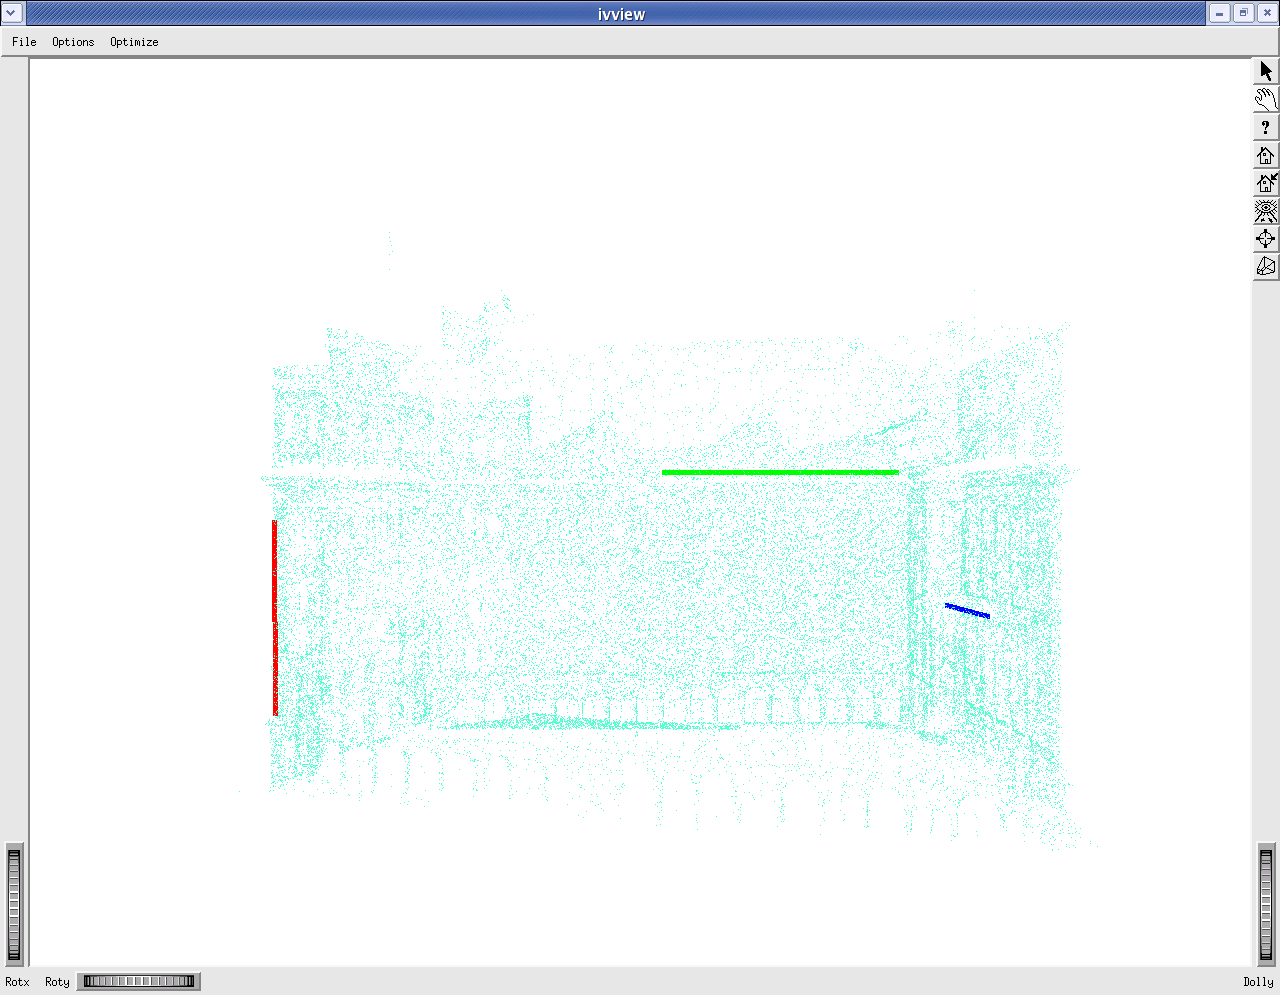
\includegraphics[width=\textwidth]{point_cloud_rectified.png}
\end{tabular}
\end{center}
\caption{ The rectified point cloud of \Fig{pc_orig}. }
\label{fig:pc_rect}
\end{figure}


%%%%

\end{document}
